% Chapter Template

\chapter{2-D Memristor Simulation} % Main chapter title

\label{Chapter6} % Change X to a consecutive number; for referencing this chapter elsewhere, use \ref{ChapterX}

\lhead{Chapter 6. \emph{Memristor Simulation}} % Change X to a consecutive number; this is for the header on each page - perhaps a shortened title

\section{2-D Memristor Model}


After creating a method to solve drift diffusion equations using finite difference in chapter 4 and testing it in chapter 5 we can now simulate an actual memristor. The most basic memristor structure consists of a rectangular strip of PEDOT with metal/carbon contacts on both sides. On top of the strip there is a drop of electrolyte solution. In order to be able to simulate the memristor we first need to determine boundary conditions and values, initial conditions and physical constans for this device.

We have two different materials and three charge carriers that are important for this problem. The drop of electrolyte has lithium and perchlorate ions and PEDOT has holes and electrons. All the carriers are not free to move everywhere. Due to PEDOT's conduction mechanism the electrons are fixed in place and holes are mobile. Also because of PEDOT's chemistry only lithium is allowed to move in so perchlorate ions always stay in the electrolyte. When a lithium ion moves into the PEDOT, through drift or diffusion, it replaces a hole. This replacement reduces the number of available holes in the PEDOT and increases its resistance. 

For the initial concentration of ions in the electrolyte we have assumed that there is no net charge and everything is uniformly distributed. Similar to electrolyte PEDOT has no net charge. All the electrons and holes are uniformly distributed and in equilibrium. Boundary conditions for all species are no flow boundary conditions with the exception of holes which can leave PEDOT through the contacts. On the contacts zero net charge is always conserved through the movement of holes in and out of the device. Lithium atoms can move between PEDOT and the electrolite but they cannot go through the contacts. Also there is a limit on the amount of lithium PEDOT can accept. Once all the holes have been replaced lithium ions cannot go into the PEDOT anymore.

The difference between the thickness of the PEDOT and electrolyte makes the simulation very difficult using uniform meshing. The thickness of the electrolyte was shortened by assuming that the amount of charge in the electrolyte is very large and more than enough to saturate PEDOT with lithium ions. Very thick electrolyte was replaced by a thinner one and the top part assumed to be an infinite source/drain for ions.

The contacts have constant potential so they have dirichlet boundary conditions. There were no constraints for the edges of the simulation domain so the potential was set to float using Neumann boundary condition.

Another important aspect of this device is the change in mobility between different materials. Lithium ions move very slowly when they get intercalated into the PEDOT. Also the regions of PEDOT that are in contact with the electrolite (wet region) has higher mobility for lithium compared to the regions that are not in contact (dry region).


\clearpage
\section{Simulation vs. Experimental Results}

\subsection{Single Channel Memristor}

In this section we will be looking into the transient simulation of a single channel memristor which is very similar to the last simulation of the previous section. Drift diffusion and Poisson's equations are coupled and lithium density is limited in PEDOT. In addition, the mobility of lithium is now gradually changing between wet and dry regions. This way lithium ions can penetrate the dry region but they cannot move too far. For transient simulation a constant potential has been applied until steady state. Once the memristor reached steady state the polarity of the potential has been switched and the simulation was run until it reached steady state. 

\begin{figure}[!htp]
\centering
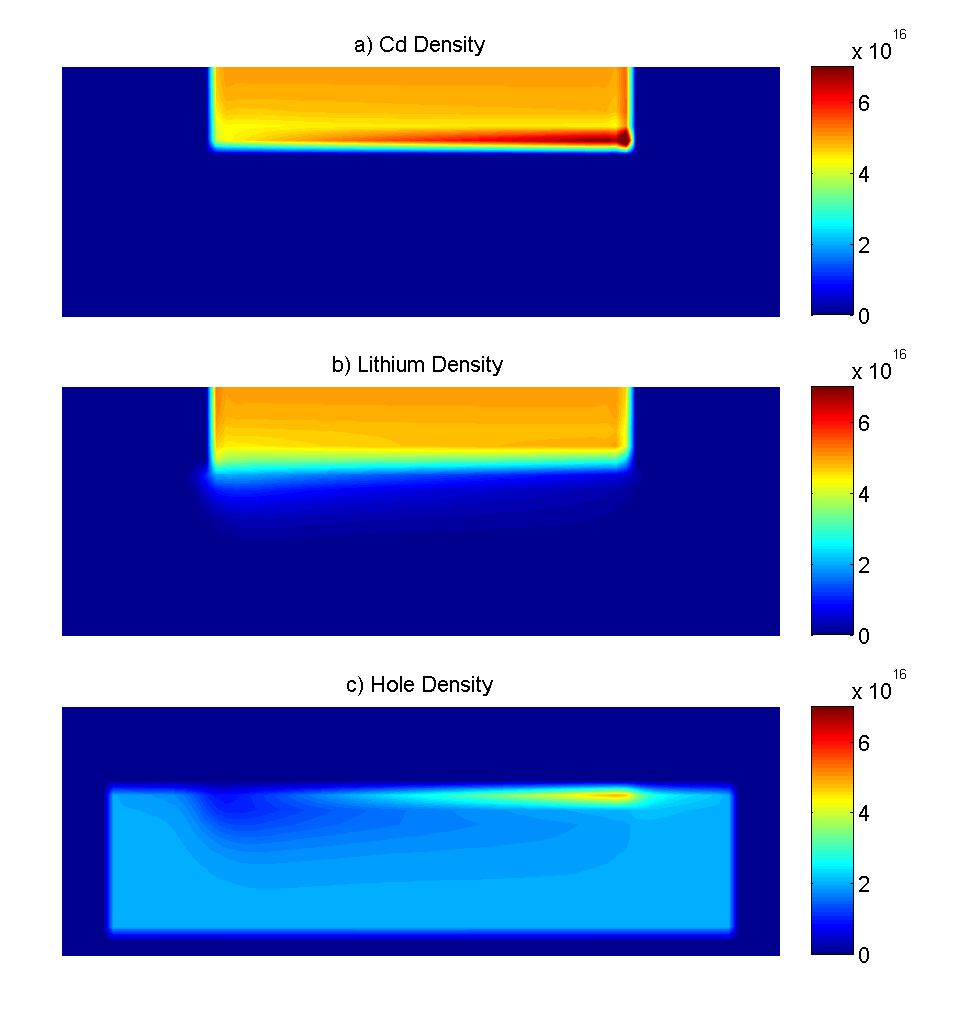
\includegraphics[scale=0.65]{Cd_Li_p_1}
\caption{Particle distribution right after the simulation has started} 
\label{Cd_Li_p_1}
\end{figure}

Following graph (\ref{Cd_Li_p_1}) shows the distribution of charged particles right after the simulation has started using initial conditions described in figure \ref{61101}. We can see that perchlorate ions quickly redistribute and pile up at the bottom right corner of the electrolyte. Lithium ions drift and diffuse into the PEDOT and move as far as they can towards the contact but they cannot reach it due to the decreased mobility in the dry region. Holes accumulate right on the interface between PEDOT and electrolyte in response to perchlorate accumulation. We can also see holes being pushed out on the left side due to the migration of lithium into PEDOT. 

At steady state we can see lithium accumulating on the left side of PEDOT and creating an area with very low hole density therefore high resistance (figure \ref{Cd_Li_p_2}). 

\begin{figure}[!htp]
\centering
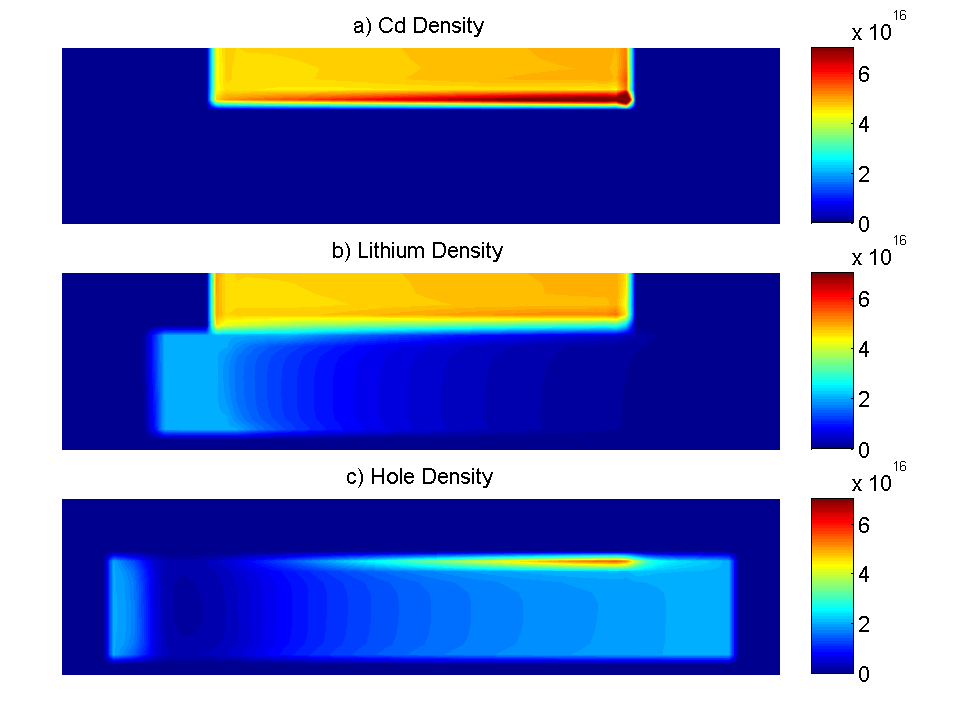
\includegraphics[scale=0.65]{Cd_Li_p_2}
\caption{Particle distribution at steady state} 
\label{Cd_Li_p_2}
\end{figure}

After the potential has been flipped (figure \ref{Cd_Li_p_3}) we can see that some lithium that got into the dry region of the PEDOT does not leave right away due to low mobility. Also, the change in potential forces lithium ions to accumulate on the right side of PEDOT.
 
\begin{figure}[!htp]
\centering
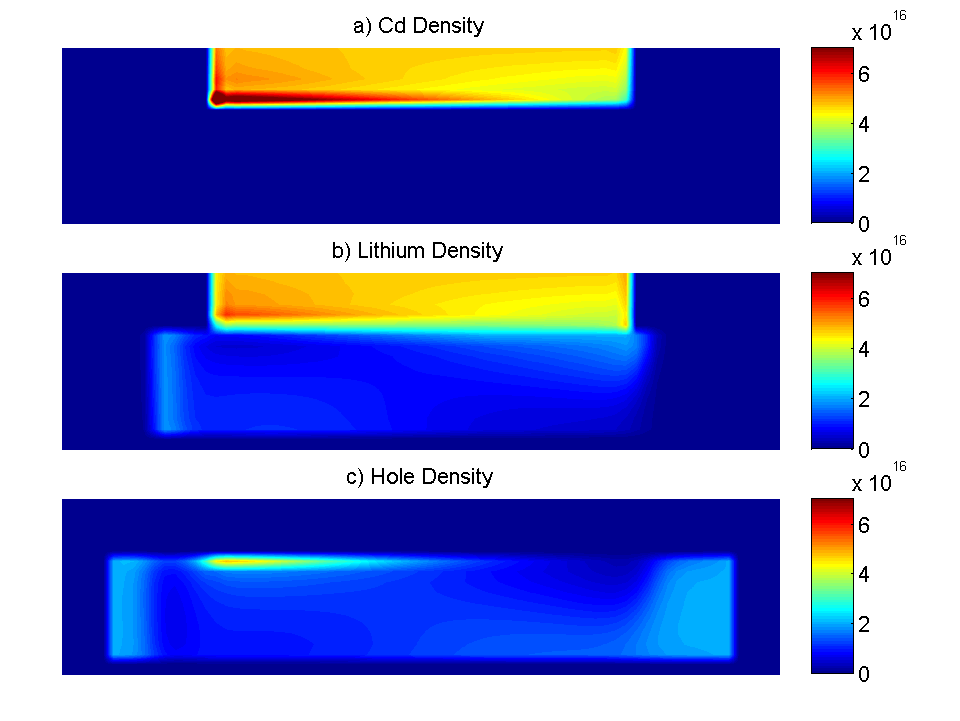
\includegraphics[scale=0.65]{Cd_Li_p_3}
\caption{Particle distribution after the potential has been changed} 
\label{Cd_Li_p_3}
\end{figure}

Finally once everything reaches steady state again almost all of the lithium ions that ware stuck in the dry region of PEDOT moved away. The final distribution for all particles looks like a mirror image of the situation with opposite potential (figure \ref{Cd_Li_p_2}). This is expected since the device is completely symmetrical.

\begin{figure}[!htp]
\centering
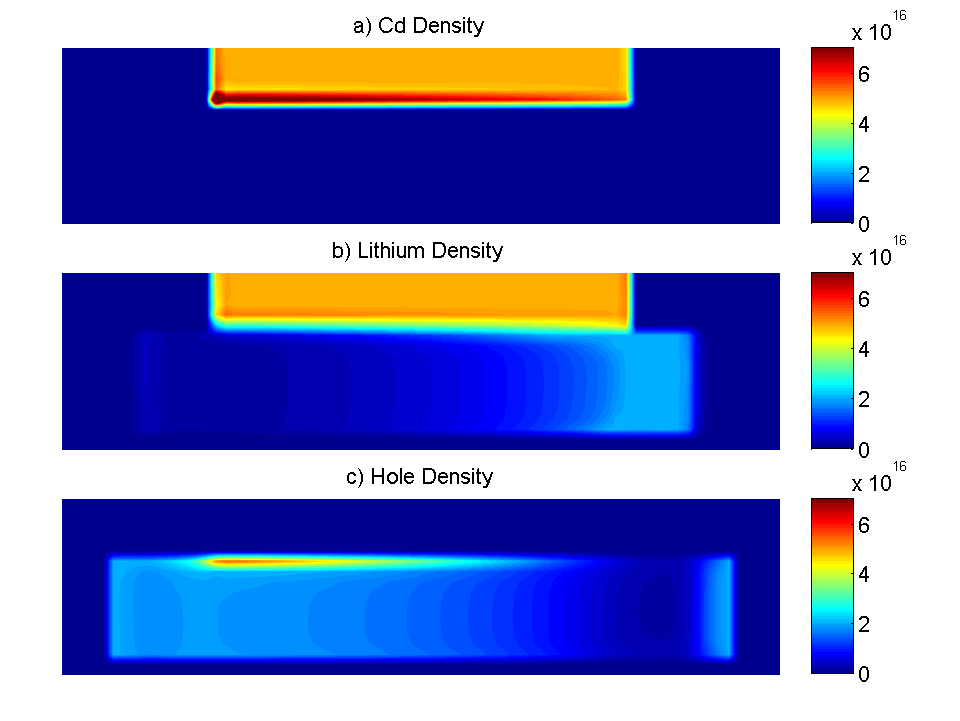
\includegraphics[scale=0.65]{Cd_Li_p_4}
\caption{Particle distribution at steady state after the potential has been changed} 
\label{Cd_Li_p_4}
\end{figure}

The next five graphs show the evolution of the potential and the electric field over time. The snapshots were taken at the same time as the ones for charged particles. The first figure (\ref{EV_0}) shows the initial potential distribution. At te second figure (\ref{EV_1}) We can see the large electric field between the PEDOT and electrolyte created by the accumulation of holes and perchlorate on both sides. Additionally the electric field inside the electrolyte is getting canceled out due to separation of charge.

\begin{figure}[!htp]
\centering
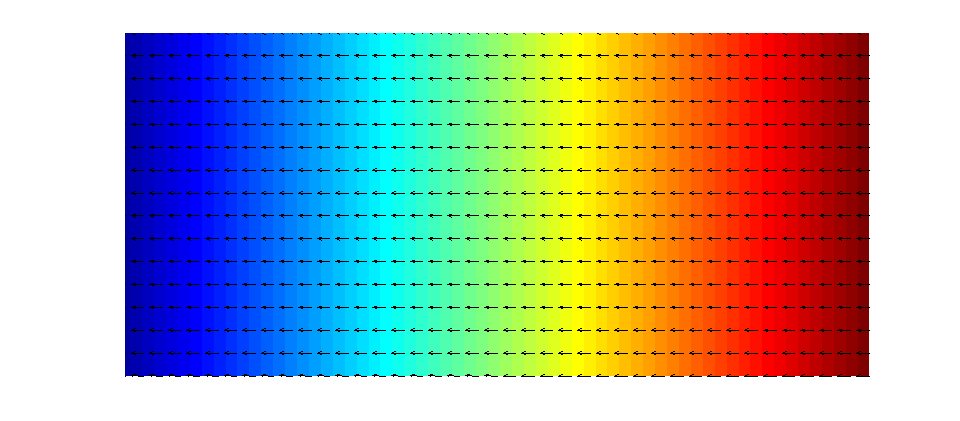
\includegraphics[scale=0.77]{EV_0}
\caption{Electric field and potential distribution before any movement of charge} 
\label{EV_0}
\end{figure}

\begin{figure}[!htp]
\centering
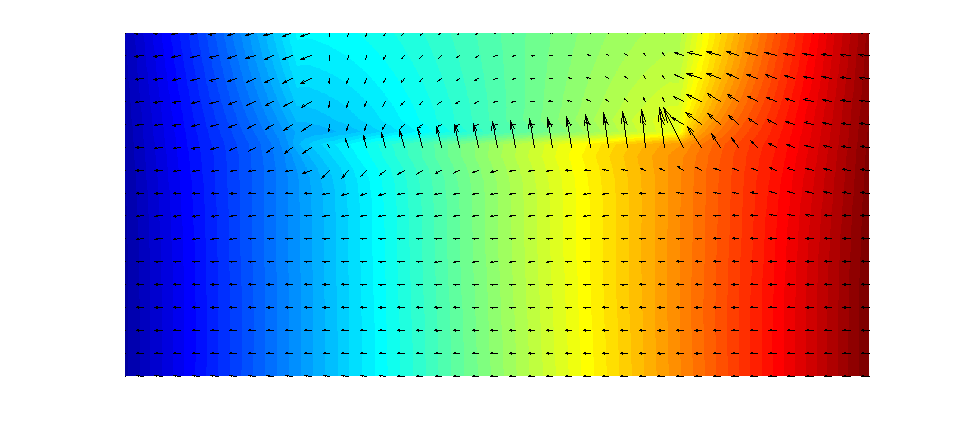
\includegraphics[scale=0.75]{EV_1}
\caption{Electric field and potential distribution right after the simulation has started} 
\label{EV_1}
\end{figure}

At steady state there is almost no electric field inside the electrolyte (figure \ref{EV_2}). Most of the electric field inside PEDOT is also canceled out by the accumulation of lithium on the left side. Almost all the electric field is concentrated around the region where lithium accumulates and forces holes out. Since the electrons are fixed in place, when holes move out they leave behind an exposed negative charge in the dry region. This strengthens the electric field even further.

\begin{figure}[!htp]
\centering
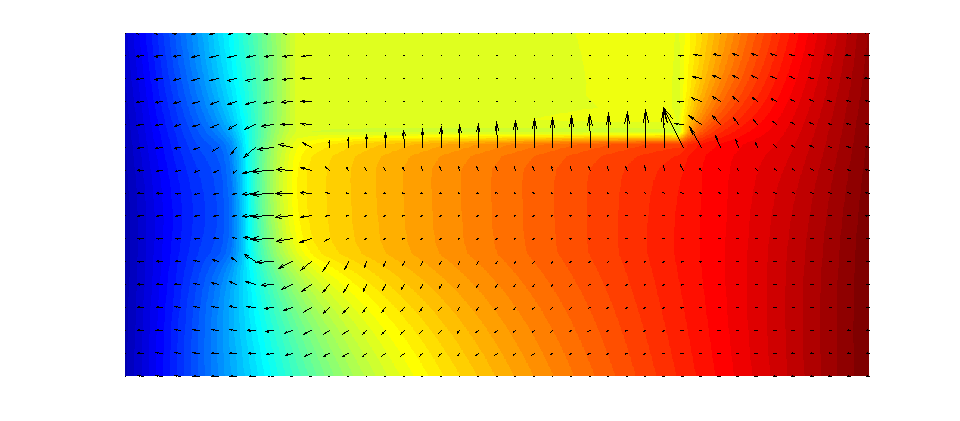
\includegraphics[scale=0.75]{EV_2}
\caption{Electric field and potential distribution at steady state} 
\label{EV_2}
\end{figure}

As soon as the potential is switched we see a change in the electric field between PEDOT and electrolyte (figure \ref{EV_3}). The electric field created by lithium on the left side of the PEDOT quickly disappears. The dark spot on the left side of PEDOT is due to lithium taking time to move towards the other side.

\begin{figure}[!htp]
\centering
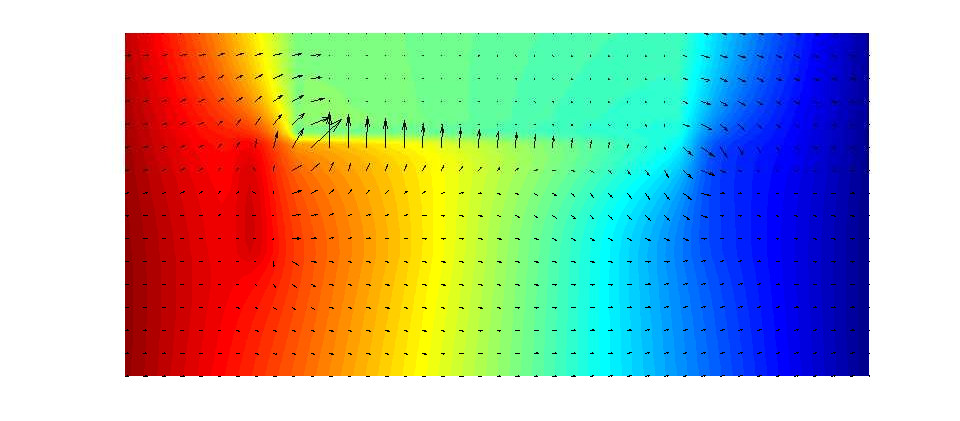
\includegraphics[scale=0.75]{EV_3}
\caption{Electric field and potential distribution right after the applied potential has been changed} 
\label{EV_3}
\end{figure}

At steady state the potential distributions of \ref{EV_2} and \ref{EV_4} are mirror images of each other except the polarity of the applied potential at the contacts are opposite. This is not unexpected since charge particle distributions had the exact same behavior. 

\begin{figure}[!htp]
\centering
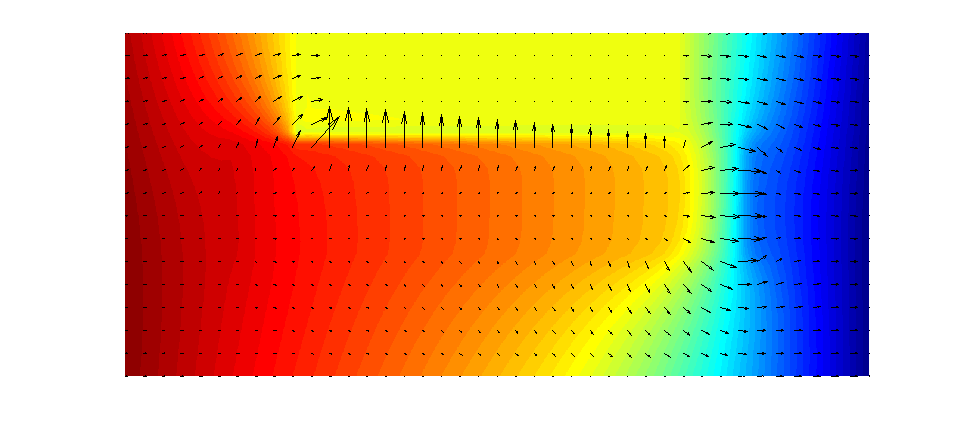
\includegraphics[scale=0.75]{EV_4}
\caption{Electric field and potential distribution at steady state after the applied potential has been changed} 
\label{EV_4}
\end{figure}

Figures \ref{Edge_1} to \ref{Edge_6} show the horizontal cross section of lithium around the wet dry/interface of PEDOT. The figures on the left side are simulation results and the figures on the right side are experimental results. Unfortunately we did not have any means of directly measuring the lithium density. The closest option to measuring lithium density in PEDOT was to capture the blue coloration of PEDOT when it interacts with lithium. This was done by recording the video of the experiment as it goes through different stages. Afterwards, the images were filtered and processed to show high values for blue and low values for other colors. 

The figure below shows the distribution of lithium right before the potential is flipped. We can see , from both simulation and experimental results, that as time progresses lithium moves towards the opposite side of the device and leaves behind a trail where mobility is very low. 

Another phenomenon that was observed in the experiment was the change in lithium penetration into dry PEDOT due to increased applied potential. The last figure in this chapter (\ref{EdgeV}) shows the maximum distance lithium travels into the dry region of PEDOT with increasing potential at the contacts. Both simulation and the experiment follow a similar trend but they deviate at higher voltages. There could be a few reasons for this discrepancy. First of all it is very hard to get an exact function for the change between wet and dry regions through experimentation so any function used to model this gradual change had to be optimized by trial and error. Since the simulation for every data point takes a very long time to run, it is very difficult to find a general function that fits all the data points. Also the grid used to simulate this problem was quite coarse so there were only a few points to represent the change between two regions.

\begin{figure}[!htp]
\centering
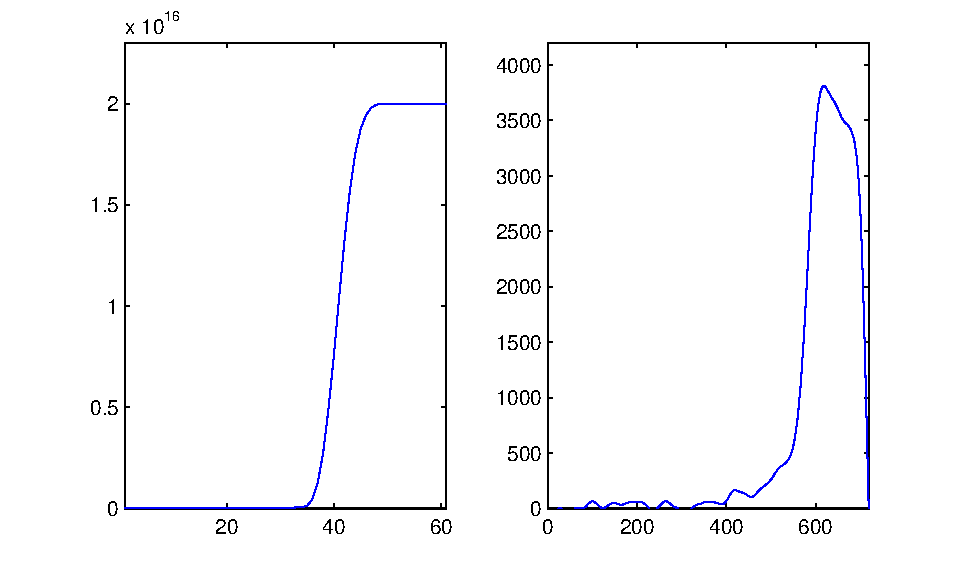
\includegraphics[scale=0.75]{Edge_1}
\caption{Lithium movement at wet/dry interface} 
\label{Edge_1}
\end{figure}

\begin{figure}[!htp]
\centering
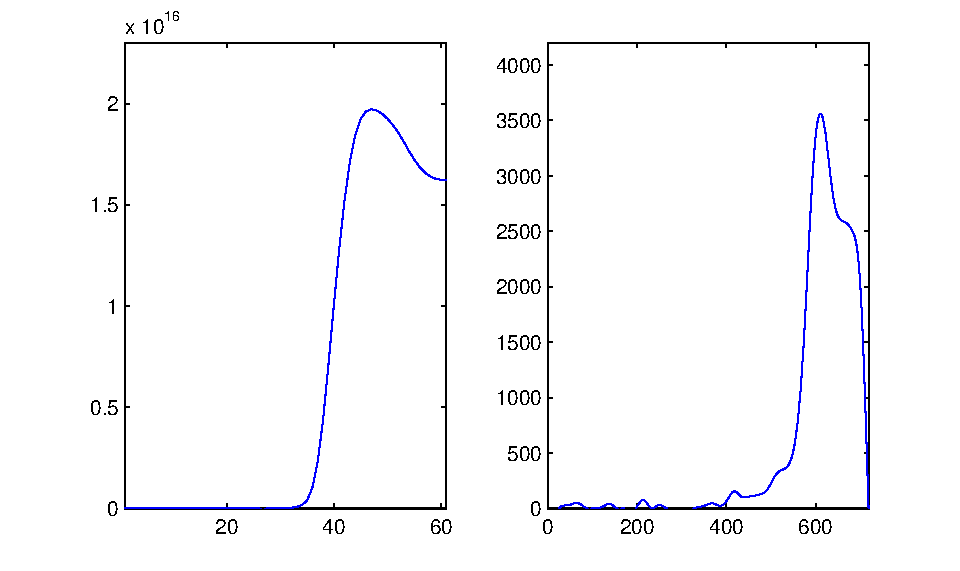
\includegraphics[scale=0.75]{Edge_2}
\caption{Lithium movement at wet/dry interface} 
\label{Edge_2}
\end{figure}

\begin{figure}[!htp]
\centering
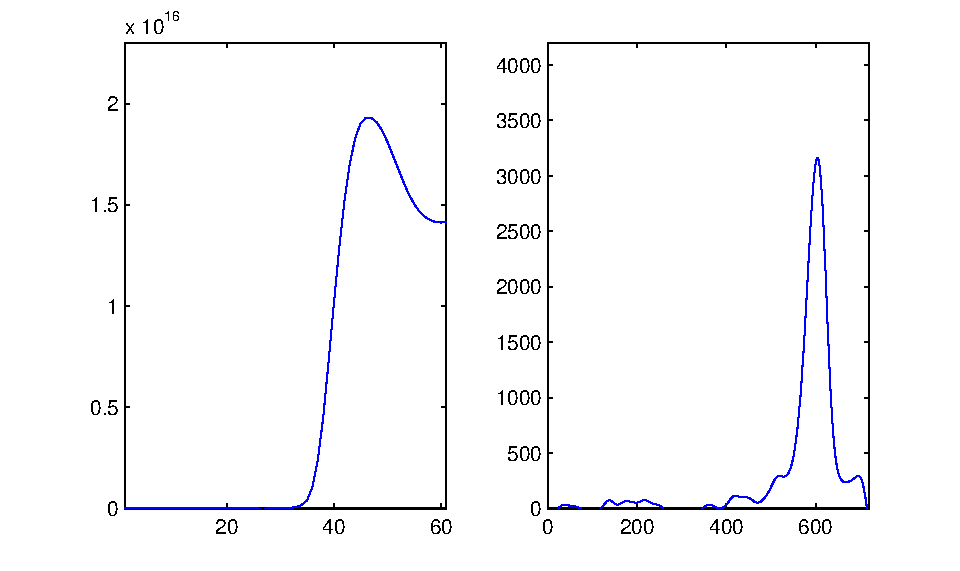
\includegraphics[scale=0.75]{Edge_3}
\caption{Lithium movement at wet/dry interface} 
\label{Edge_3}
\end{figure}


\begin{figure}[!htp]
\centering
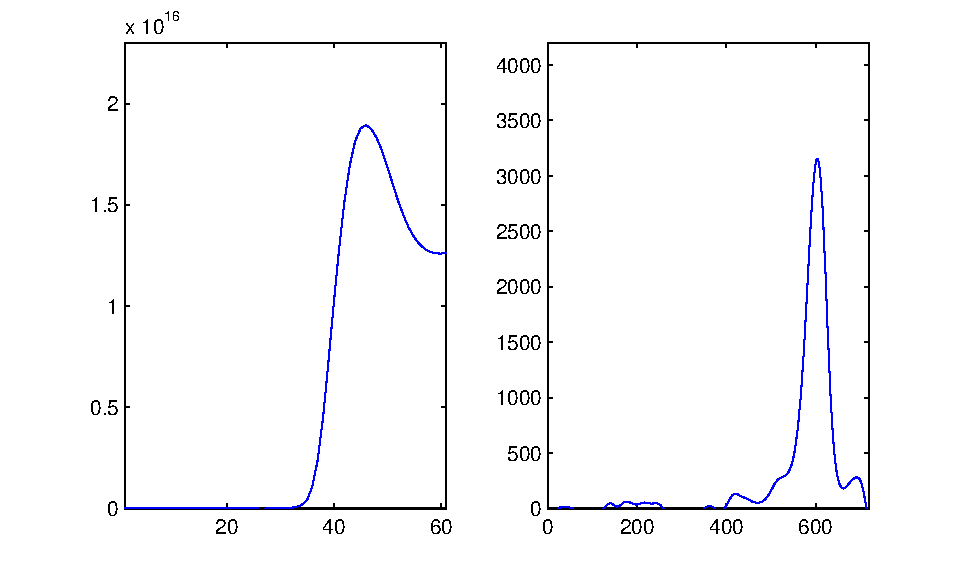
\includegraphics[scale=0.75]{Edge_4}
\caption{Lithium movement at wet/dry interface} 
\label{Edge_4}
\end{figure}

\begin{figure}[!htp]
\centering
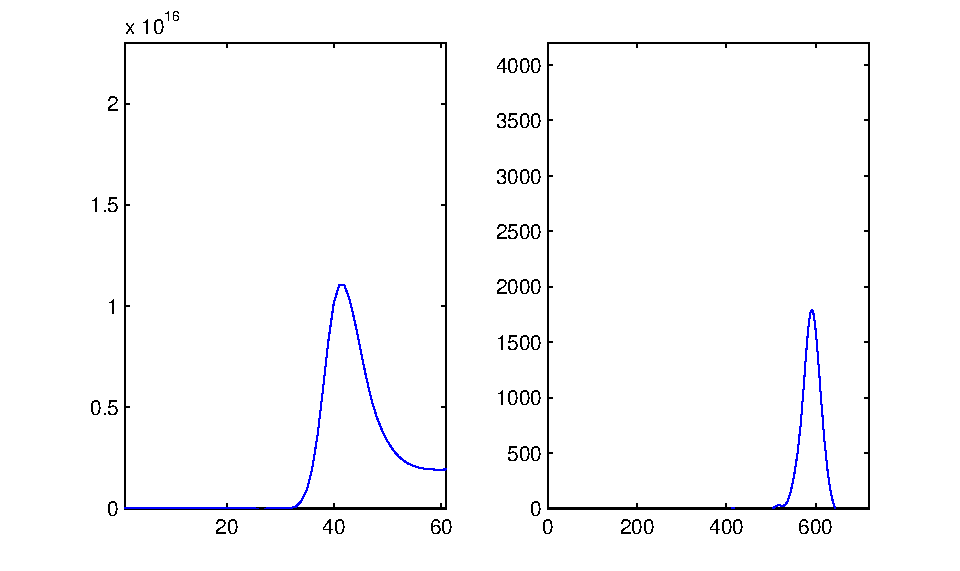
\includegraphics[scale=0.75]{Edge_5}
\caption{Lithium movement at wet/dry interface} 
\label{Edge_5}
\end{figure}

\begin{figure}[!htp]
\centering
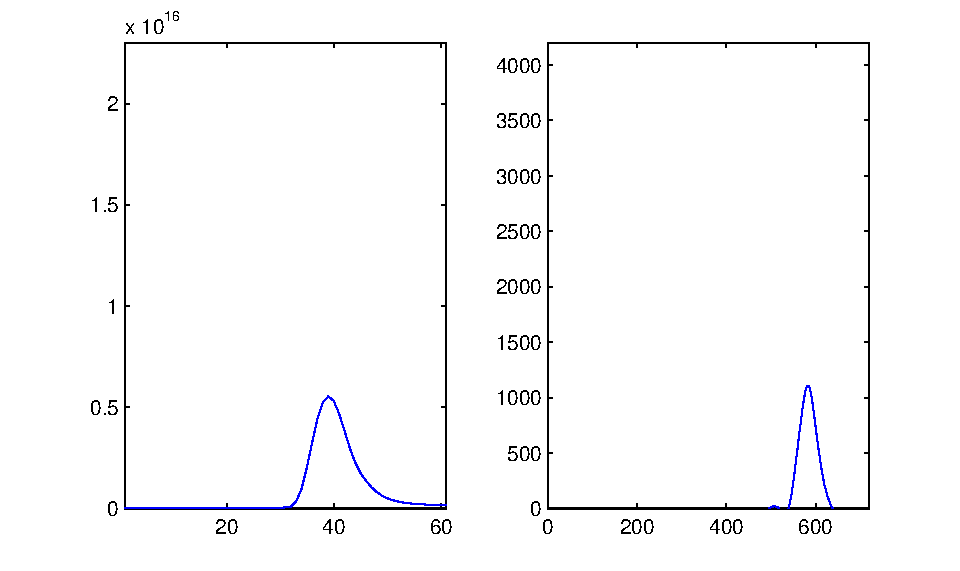
\includegraphics[scale=0.75]{Edge_6}
\caption{Lithium movement at wet/dry interface} 
\label{Edge_6}
\end{figure}

\begin{figure}[!htp]
\centering
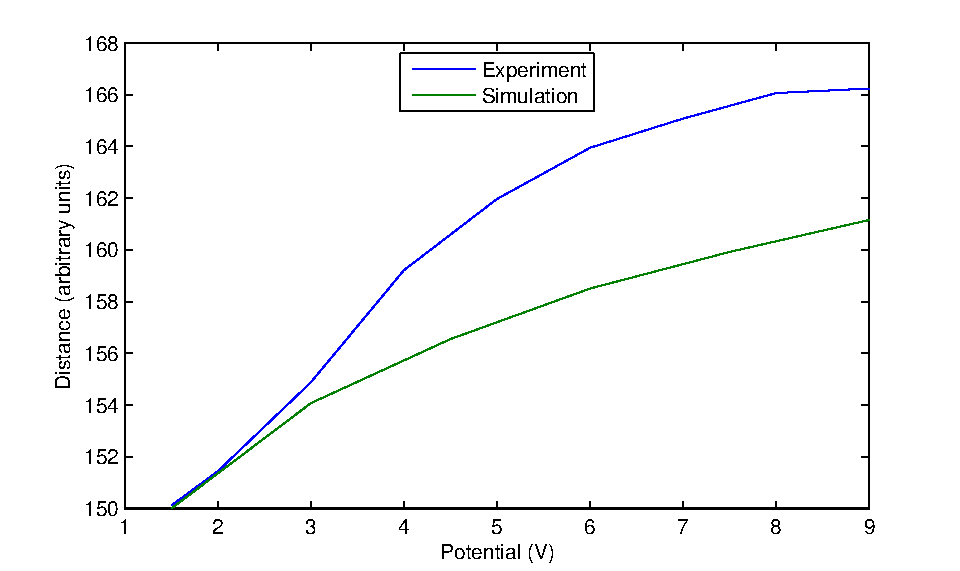
\includegraphics[scale=0.75]{EdgeV}
\caption{Penetration of lithium into dry PEDOT} 
\label{EdgeV}
\end{figure}

\clearpage
\subsection{Noteched PEDOT}

In this section we will be looking at a structure which is very similar to the single channel memristor. All the boundary conditions and initial values are the same except this time there is a notch in the PEDOT (figure \ref{NCd_Li_p_0}). So there is no hole current through the device and lithium cannot migrate into the notch. The device itself has very limited practical use but the experimental results are very suitable to test our numerical model. 

\begin{figure}[!htp]
\centering
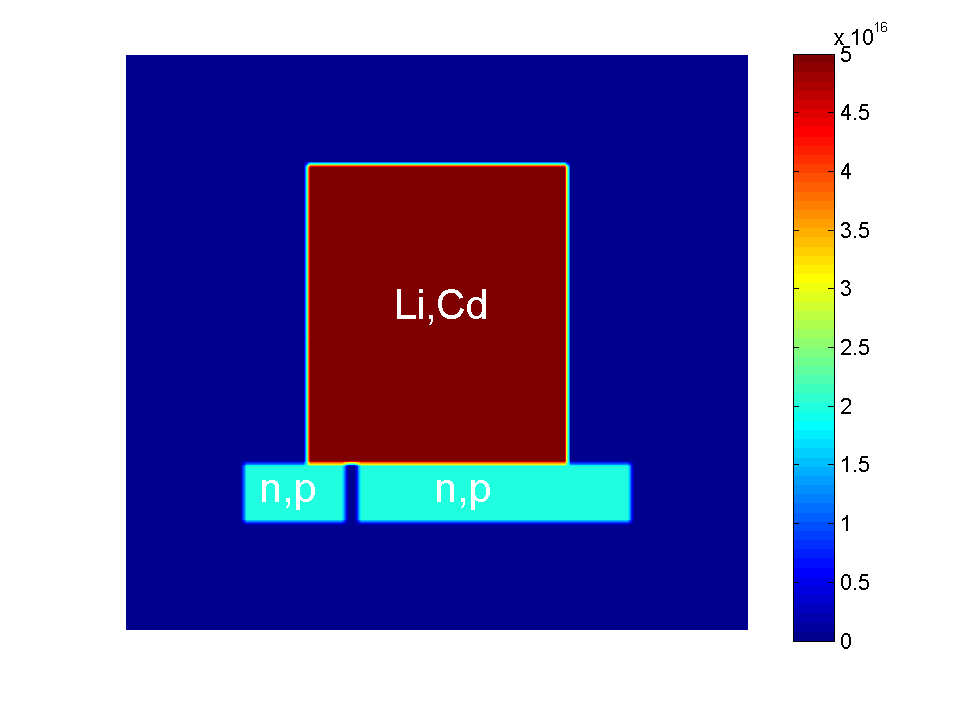
\includegraphics[scale=0.9]{NCd_Li_p_0}
\caption{Initial hole, electron, perchlorate and lithium distribution for a notched memristor} 
\label{NCd_Li_p_0}
\end{figure}

The notch in the PEDOT is sandwiched between two conductive parts. This is analogous to having a simple circuit with two low and one high resistance in series. Based on this analogy we can see that almost all the potential drop is going to be on the notch. One side of the PEDOT will have a low potential and the other side will have a high potential. In figure \ref{NCD_Li_p_1} we can see lithium slowly moving towards the negative side of the PEDOT. At the same time perchlorate is starting to accumulate on the positive side. We can also see a significant hole accumulation inside PEDOT right before the notch. 

\begin{figure}[!htp]
\centering
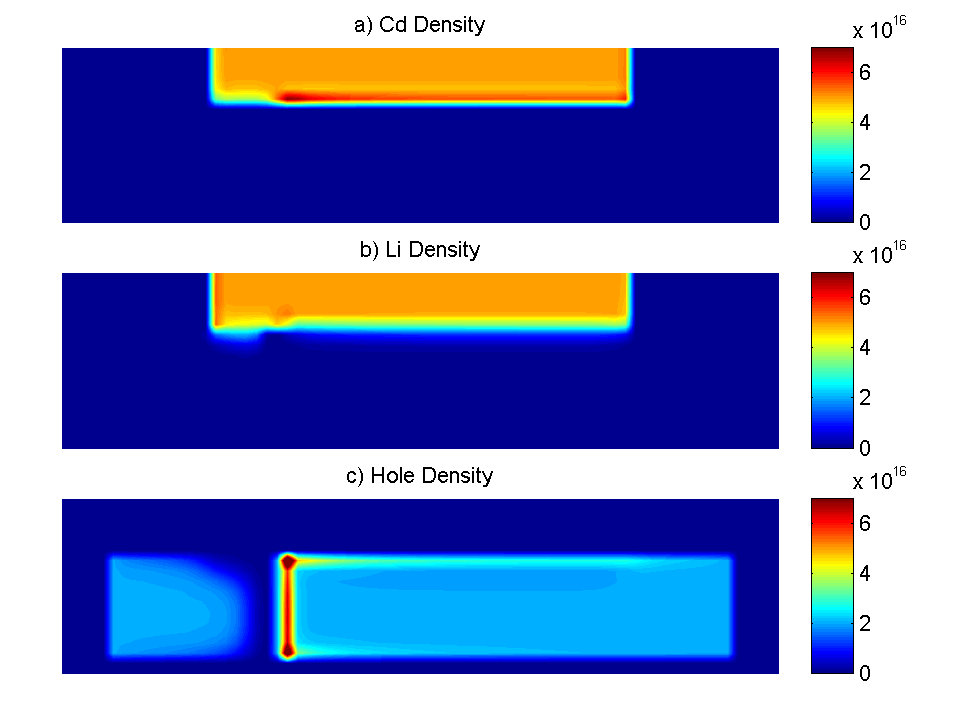
\includegraphics[scale=0.7]{NCd_Li_p_1}
\caption{Particle distribution shortly after the simulation has started} 
\label{NCD_Li_p_1}
\end{figure}

As time goes by more lithium is pushed away from the positive side of the PEDOT and pulled into the negative side (figure \ref{NCD_Li_p_2}). The here is a noticeable lack of lithium on the side with positive contact at the electrolyte/PEDOT interface. While lithium is pulled into the PEDOT holes are being pushed away. Holes also accumulate at the surface of the PEDOT due to accumulation of perchlorate right across the interface.

\begin{figure}[!htp]
\centering
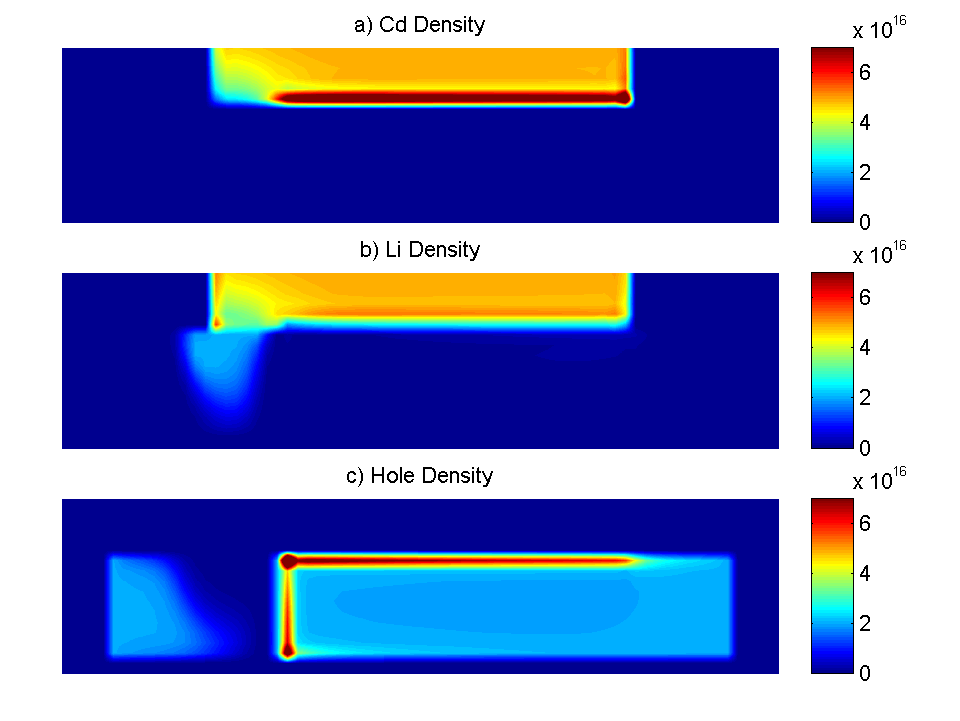
\includegraphics[scale=0.7]{NCd_Li_p_2}
\caption{Particle distribution before steady state} 
\label{NCD_Li_p_2}
\end{figure}

At steady state we can see that lithium density in PEDOT is uniform and at its maximum value (\ref{NCd_Li_p_3}). At the same area we can see the lack of holes due to migration of lithium.
 
\begin{figure}[!htp]
\centering
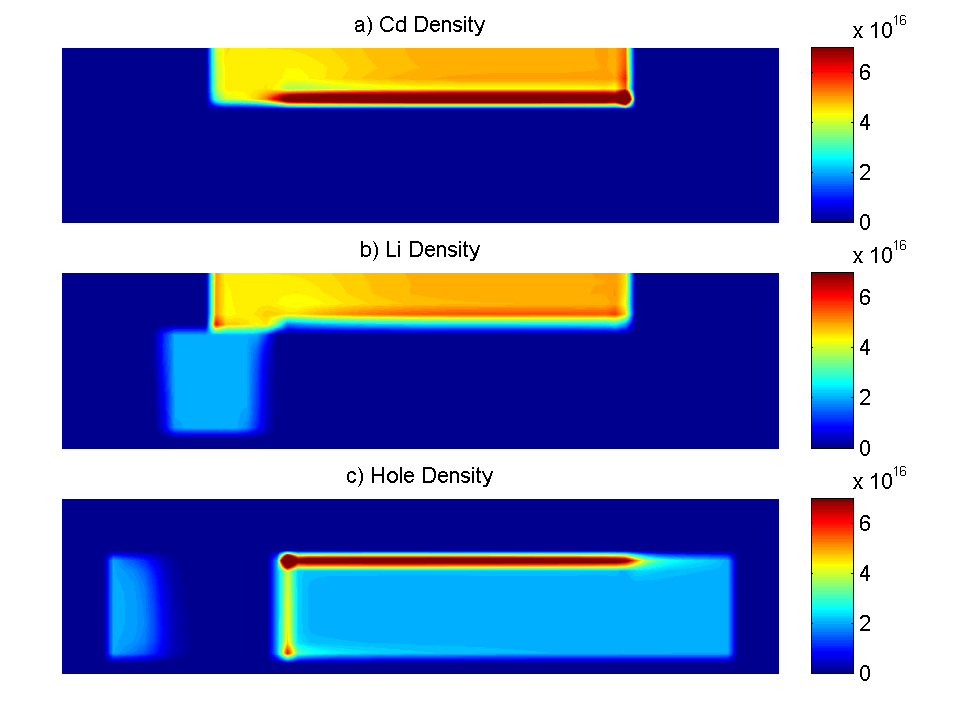
\includegraphics[scale=0.7]{NCd_Li_p_3}
\caption{Particle distribution at steady state} 
\label{NCd_Li_p_3}
\end{figure}

Once the potential is flipped everything starts to move in opposite direction (figures \ref{NCd_Li_p_4} and \ref{NCd_Li_p_5}). Perchlorate moves towards the positive contact. Lithium ions start to leave the PEDOT on the left side of the notch and they get attracted towards the right side. Holes start to accumulate on the left side instead of the right side.

In figure \ref{NCd_Li_p_5} we can see that due to the strength of the electric field, holes and perchlorate ions gather on the left side of the PEDOT/electrolyte interface very quickly and leave behind a depleted region. Also as lithium settles in the right side of the PEDOT holes start to move away.

\begin{figure}[!htp]
\centering
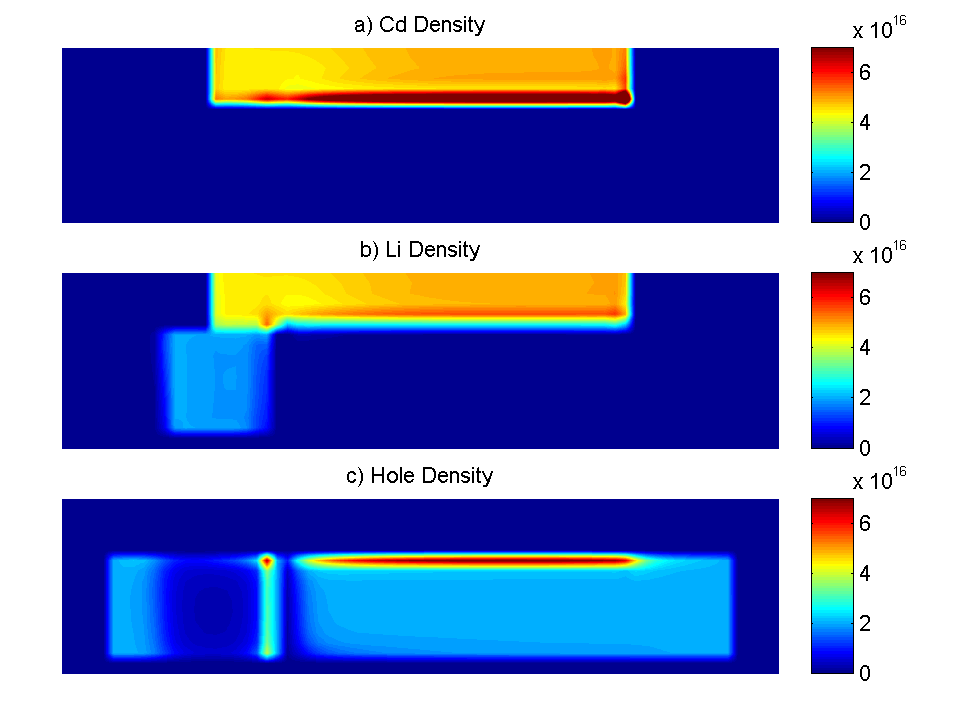
\includegraphics[scale=0.70]{NCd_Li_p_4}
\caption{Particle distribution right after applied potential has been switched} 
\label{NCd_Li_p_4}
\end{figure}

\begin{figure}[!htp]
\centering
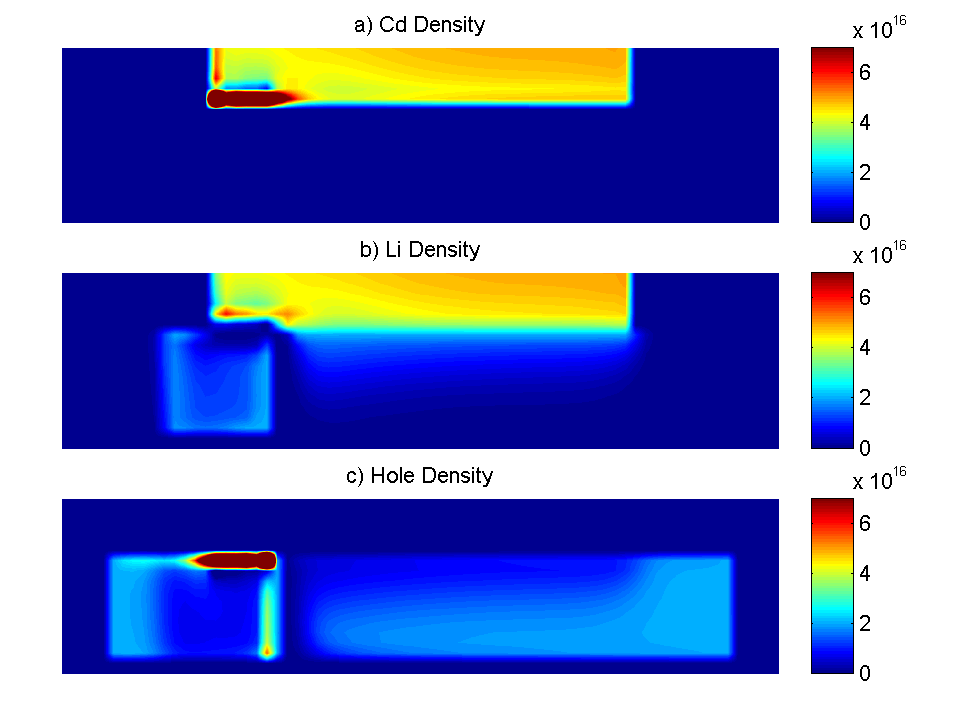
\includegraphics[scale=0.70]{NCd_Li_p_5}
\caption{Particle distribution close to steady state after the potential has been switched} 
\label{NCd_Li_p_5}
\end{figure}

Steady state in figure \ref{NCd_Li_p_6} is the complete opposite of figure \ref{NCd_Li_p_3}. The potential is flipped therefore everything else appears on the opposite side. In both cases lithium ions push out holes and perchlorate accumulates at the interface.

\begin{figure}[!htp]
\centering
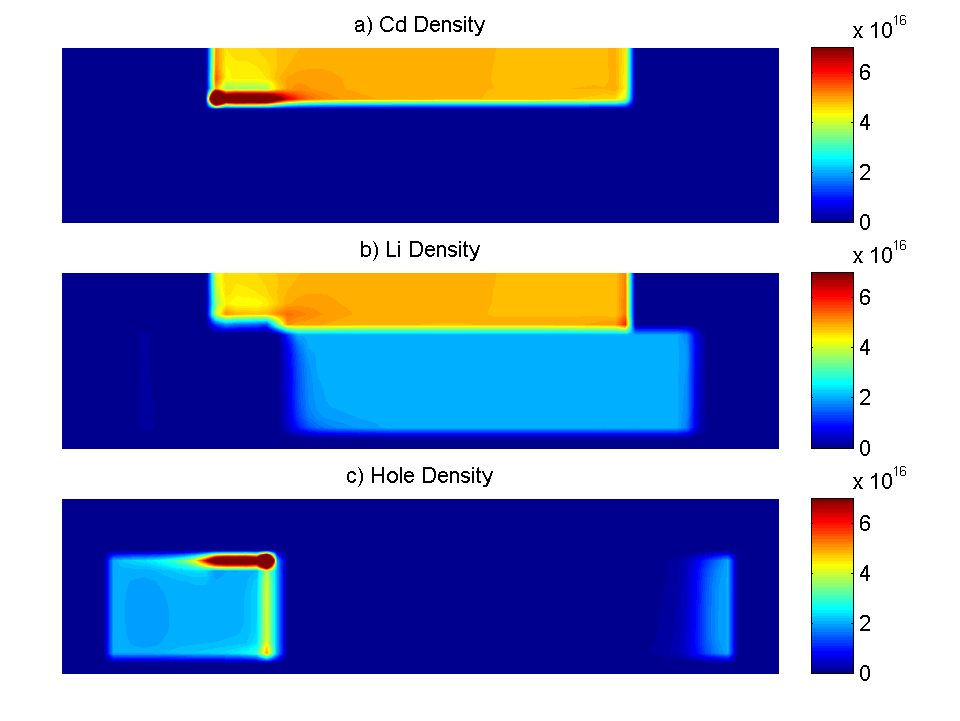
\includegraphics[scale=0.7]{NCd_Li_p_6}
\caption{Particle distribution at steady state after the potential has been switched} 
\label{NCd_Li_p_6}
\end{figure}

Figures \ref{NEV_0} to \ref{NEV_6} show the evolution of electric field and potential over time. Right after the simulation has started we can see a large drop of potential and a large electric field at the gap (figure \ref{NEV_1}). There is also a large electric field forming at the PEDOT/electrolyte interface as holes and perchlorate ions right across each other.

\begin{figure}[!htp]
\centering
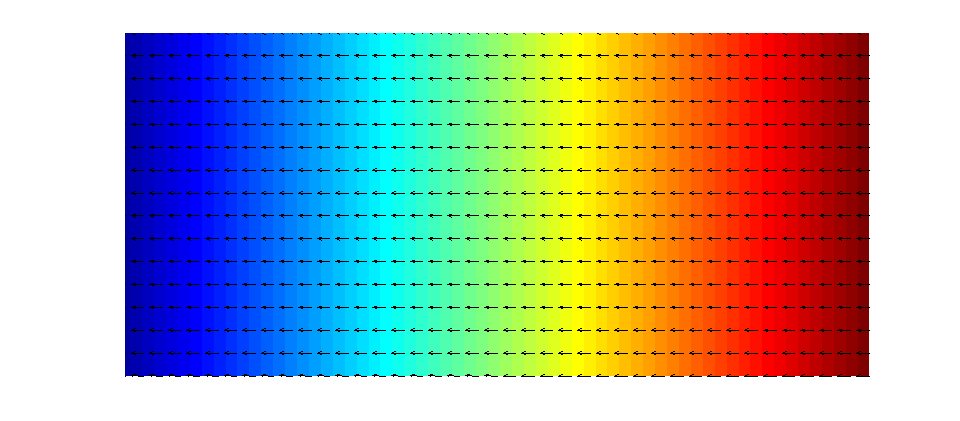
\includegraphics[scale=0.8]{NEV_0}
\caption{Electric field and potential distribution before redistribution of charge} 
\label{NEV_0}
\end{figure}

\begin{figure}[!htp]
\centering
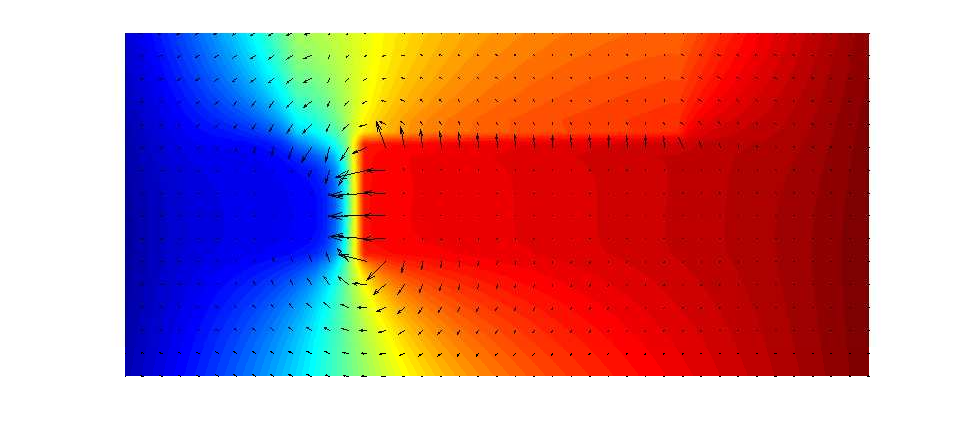
\includegraphics[scale=0.8]{NEV_1}
\caption{Electric field and potential distribution shortly after the simulation has started} 
\label{NEV_1}
\end{figure}
In figure \ref{NEV_2} we can see the cancellation of the electric field inside the electrolyte due to redistribution of charge. We can also see the effect of lithium ions moving in on the left corner of the notch.

\begin{figure}[!htp]
\centering
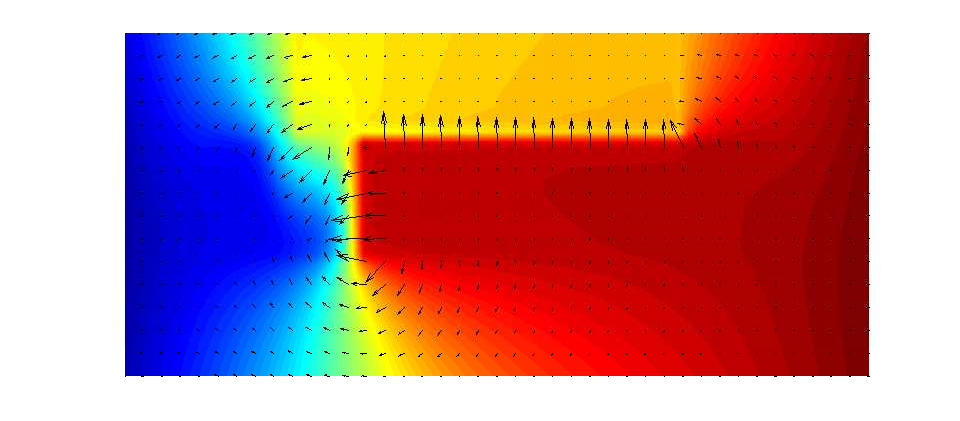
\includegraphics[scale=0.8]{NEV_2}
\caption{Electric field and potential distribution before steady state} 
\label{NEV_2}
\end{figure}

At steady state we can see that the electric field on the right side of the notch was canceled but there is still an electric field on the left side (figure \ref{NEV_3}). This is due to the density limit of lithium. Holes cannot accumulate at the contact and lithium can only accumulate until a certain density so the electric field in that region does not get canceled out.

\begin{figure}[!htp]
\centering
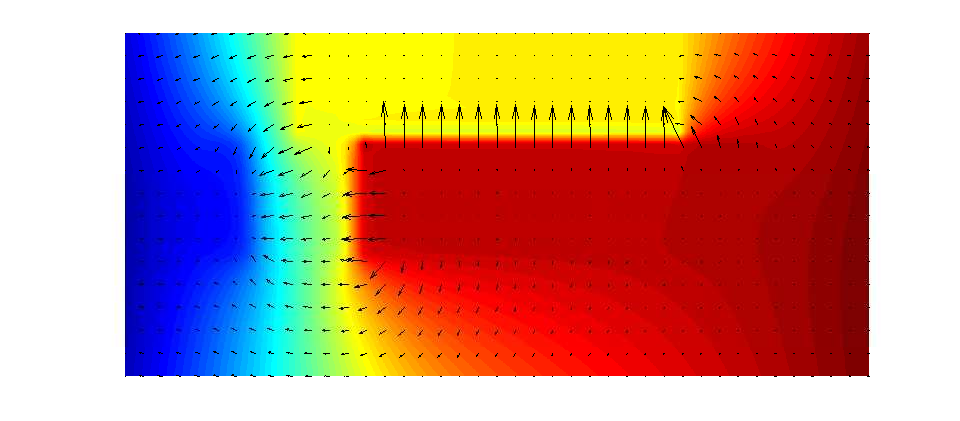
\includegraphics[scale=0.8]{NEV_3}
\caption{Electric field and potential distribution at steady state} 
\label{NEV_3}
\end{figure}

The same process repeats itself after the applied potential has been switched (figures \ref{NEV_4} to \ref{NEV_6} ). Holes accumulate on the left side of the notch and cancel the electric field. Also there is a large electric field emerges due to the accumulation of perchlorate ions and holes at the boundaries on the left side (figure \ref{NEV_6}).

\begin{figure}[!htp]
\centering
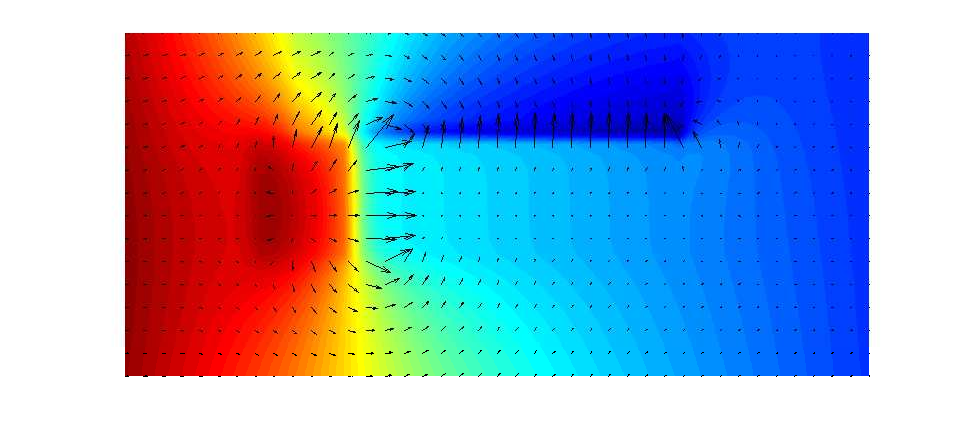
\includegraphics[scale=0.82]{NEV_4}
\caption{Electric field and potential distribution right after applied potential has been switched} 
\label{NEV_4}
\end{figure}

\begin{figure}[!htp]
\centering
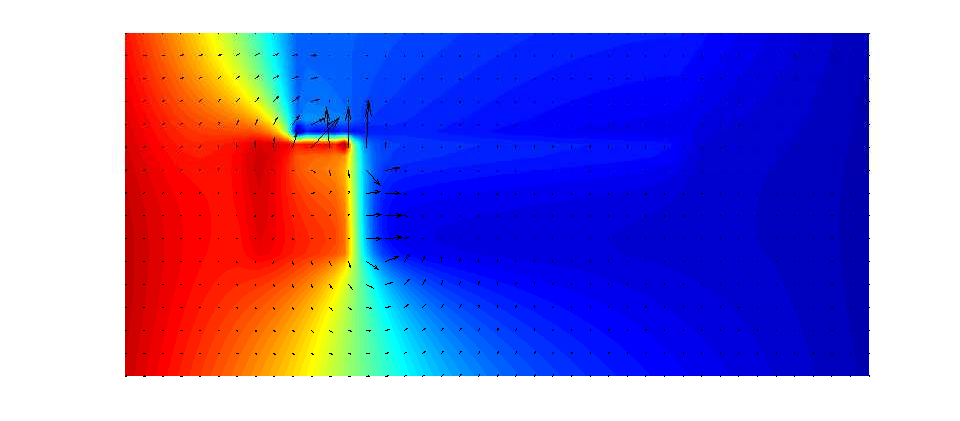
\includegraphics[scale=0.82]{NEV_5}
\caption{Electric field and potential distribution before steady state} 
\label{NEV_5}
\end{figure}

\begin{figure}[!htp]
\centering
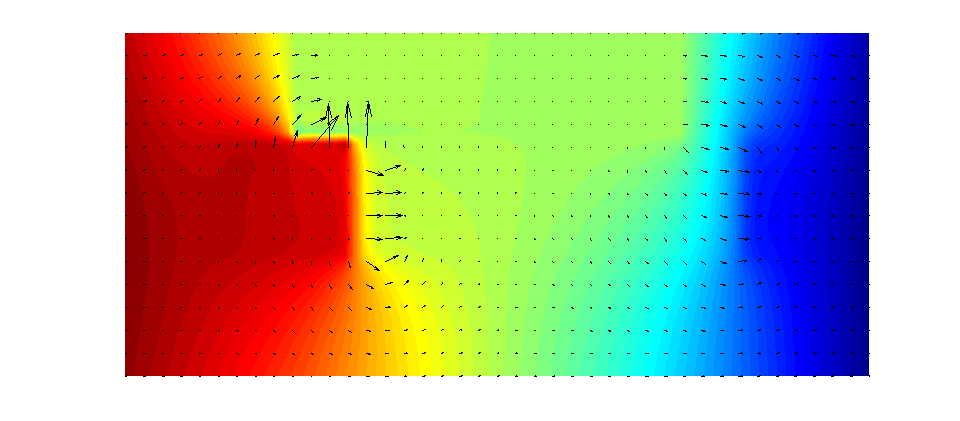
\includegraphics[scale=0.82]{NEV_6}
\caption{Electric field and potential distribution at steady state} 
\label{NEV_6}
\end{figure}

The only experimental measurement directly showing the movement of lithium ions inside is the video showing the blue coloration of PEDOT. Figures \ref{Front_1} to \ref{Front_12} compare the simulation lithium movement with experimental results. Following figures show a horizontal cross section of PEDOT (only the side that is receiving lithium)near the electrolyte. The experimental results show the blue coloration of PEDOT after some filtering and image processing. High values in the y axis of signify blue coloration and low values are other colors. 

In both experiment and simulation lithium ions start to move in from the notched side. As time progresses lithium ions move toward the contact. There are two effects contributing to this behavior. The electric field is at its highest right around the notch. So this is where the most amount of lithium is pulled into PEDOT. As lithium ions move in vertically, they drift horizontally through PEDOT due to electric field created by the contacts.

When ion movement approaches steady state, in the experiment, we can see that coloration becomes more uniform and stops changing. In the simulation lithium reaches its maximum density and PEDOT stops receiving any additional ions. Overall the behavior seen in this simulation matches the experimental observations quite well. 
 
\begin{figure}[!htp]
\centering
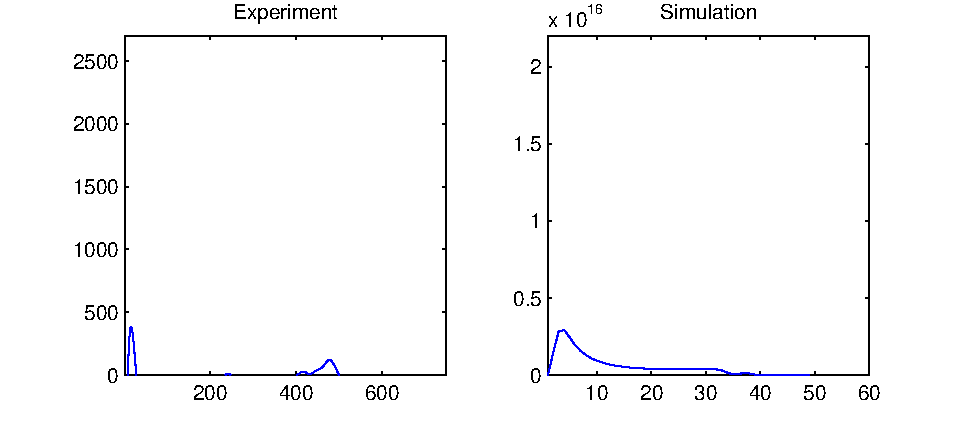
\includegraphics[scale=0.8]{Front_1}
\caption{Movement of lithium ions into PEDOT} 
\label{Front_1}
\end{figure}

\begin{figure}[!htp]
\centering
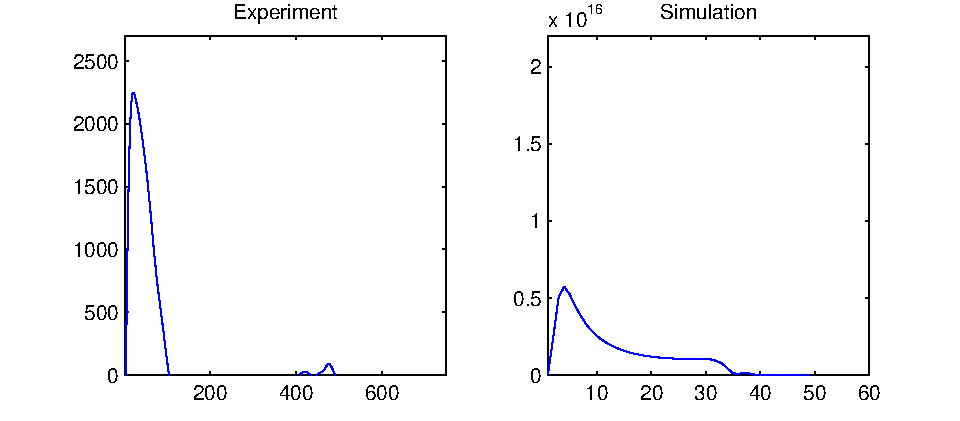
\includegraphics[scale=0.8]{Front_2}
\caption{Movement of lithium ions into PEDOT} 
\label{Front_2}
\end{figure}

\begin{figure}[!htp]
\centering
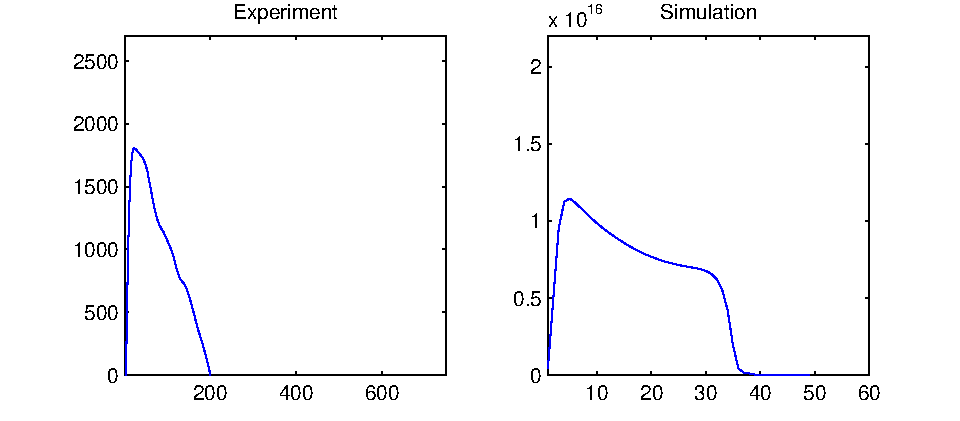
\includegraphics[scale=0.8]{Front_3}
\caption{Movement of lithium ions into PEDOT} 
\label{Front_3}
\end{figure}

\begin{figure}[!htp]
\centering
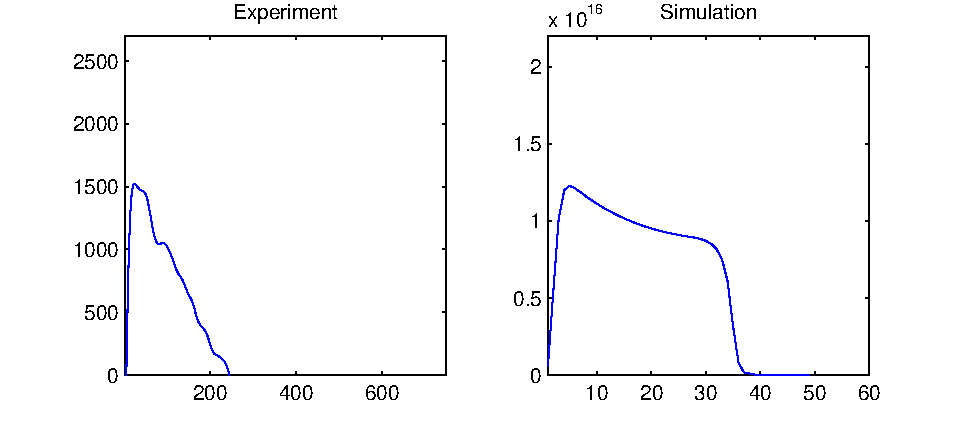
\includegraphics[scale=0.8]{Front_4}
\caption{Movement of lithium ions into PEDOT} 
\label{Front_4}
\end{figure}

\begin{figure}[!htp]
\centering
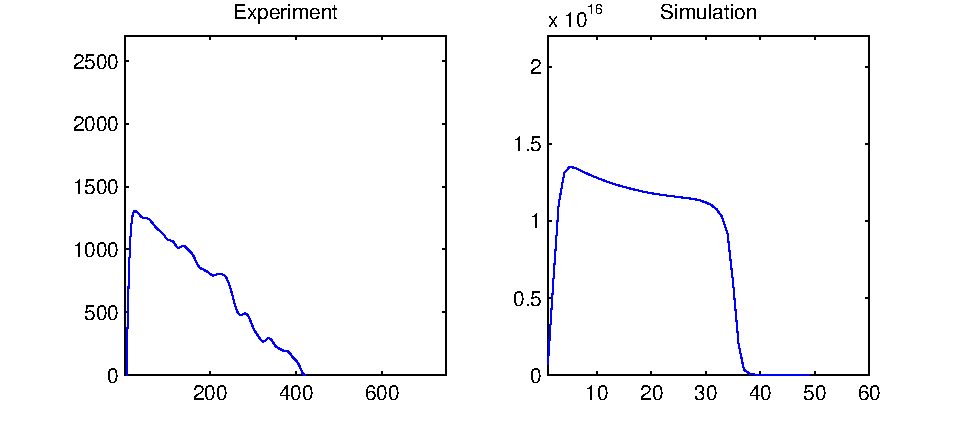
\includegraphics[scale=0.8]{Front_5}
\caption{Movement of lithium ions into PEDOT} 
\label{Front_5}
\end{figure}

\begin{figure}[!htp]
\centering
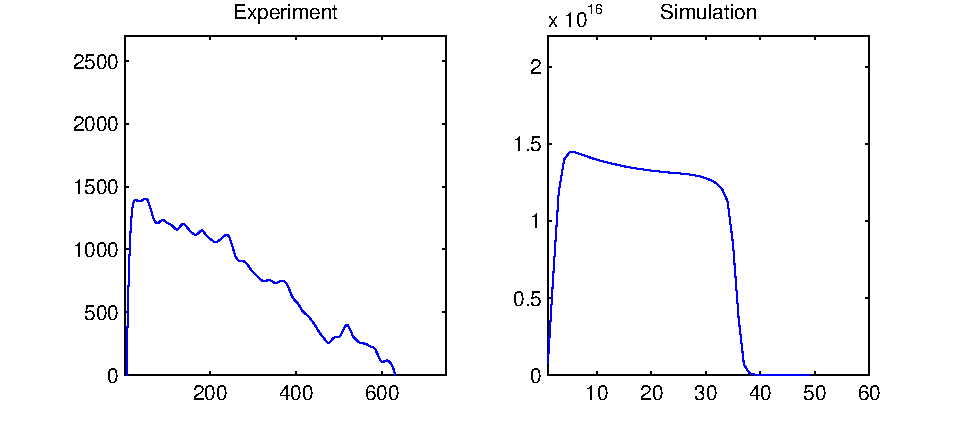
\includegraphics[scale=0.8]{Front_6}
\caption{Movement of lithium ions into PEDOT} 
\label{Front_6}
\end{figure}

\begin{figure}[!htp]
\centering
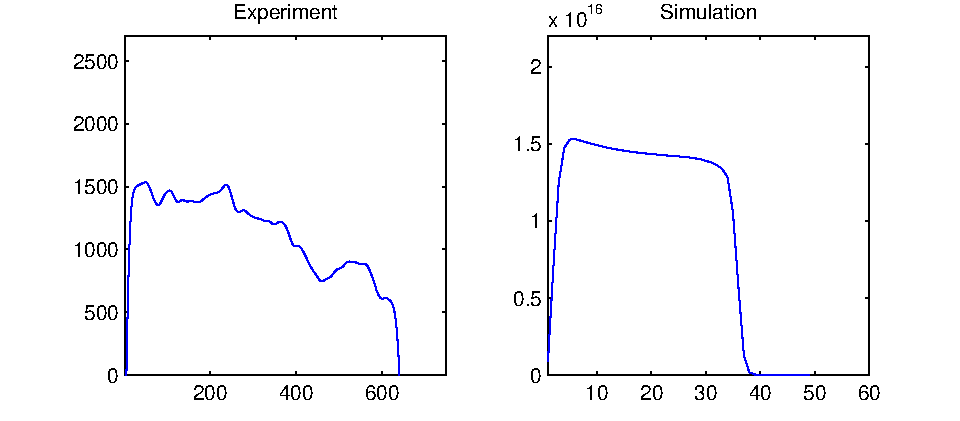
\includegraphics[scale=0.8]{Front_7}
\caption{Movement of lithium ions into PEDOT} 
\label{Front_7}
\end{figure}

\begin{figure}[!htp]
\centering
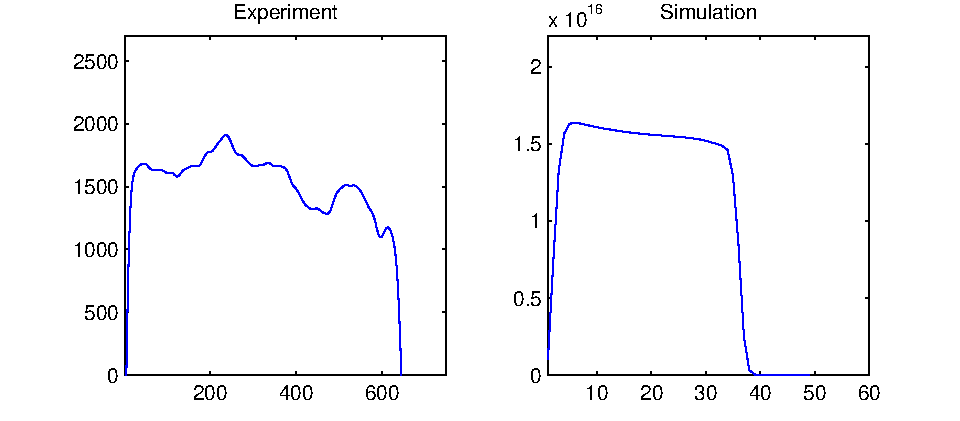
\includegraphics[scale=0.8]{Front_8}
\caption{Movement of lithium ions into PEDOT} 
\label{Front_8}
\end{figure}

\begin{figure}[!htp]
\centering
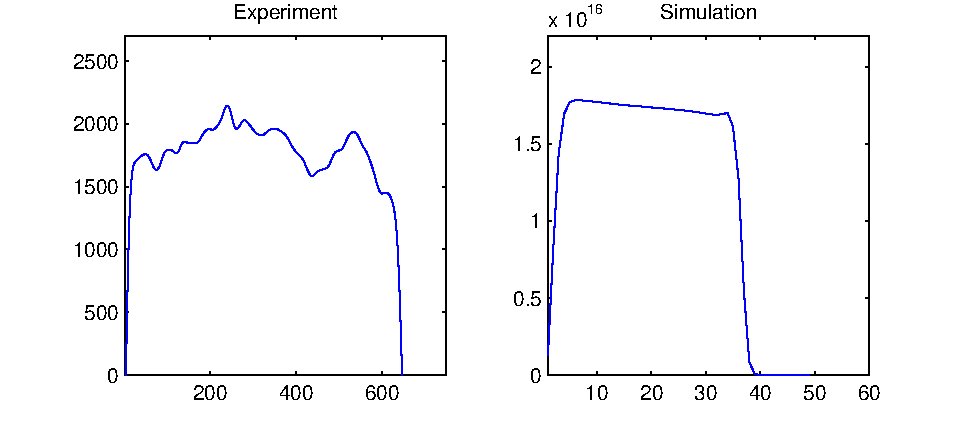
\includegraphics[scale=0.8]{Front_9}
\caption{Movement of lithium ions into PEDOT} 
\label{Front_9}
\end{figure}

\begin{figure}[!htp]
\centering
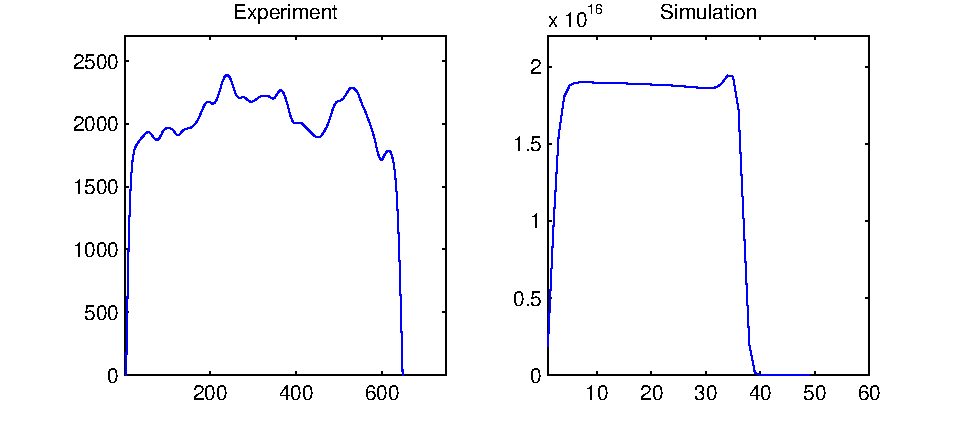
\includegraphics[scale=0.8]{Front_10}
\caption{Movement of lithium ions into PEDOT} 
\label{Front_10}
\end{figure}

\begin{figure}[!htp]
\centering
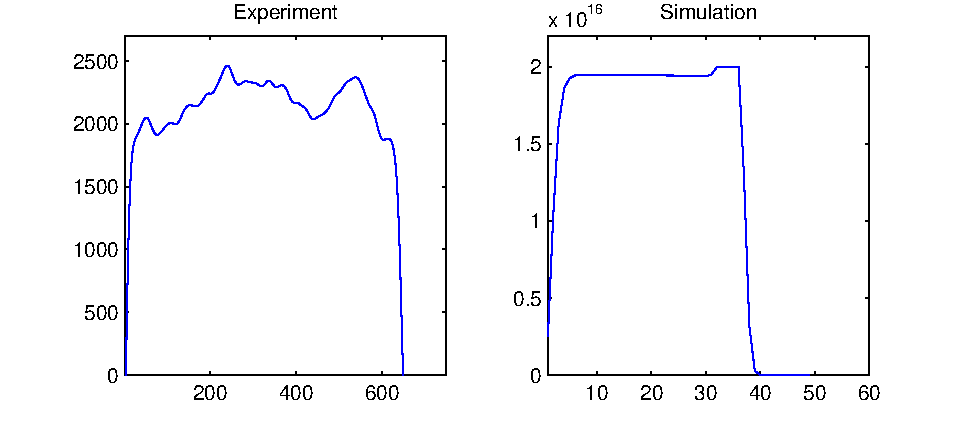
\includegraphics[scale=0.8]{Front_11}
\caption{Movement of lithium ions into PEDOT} 
\label{Front_11}
\end{figure}

\begin{figure}[!htp]
\centering
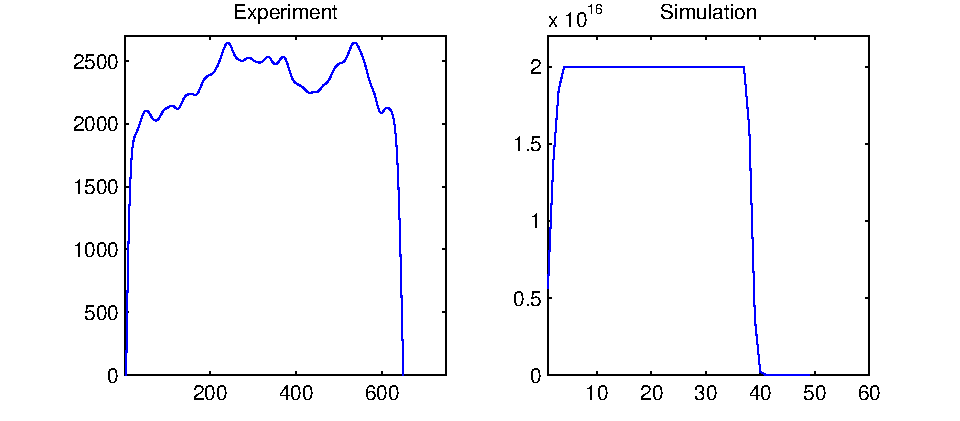
\includegraphics[scale=0.8]{Front_12}
\caption{Movement of lithium ions into PEDOT} 
\label{Front_12}
\end{figure}